\chapter{Naughty maid}
Naughty maid is the adult theme app name of the remaining four malware samples analyzed. The objective of the virus is to log to a remote chinese server sensitive information like position and stored files and, in addition, can make the phone subscribe to paid SMS services  and cancel the SMS afterwards to hide its malicious behavior.

\section{File differences}
As previously stated we received four jar files identified by their SHA256 hash:
\begin{itemize}
	\item \texttt{0b8bae30da84fb181a9ac2b1dbf77eddc5728fab8dc5db44c11069fef1821ae6}
	\item \texttt{0b41181a6b9c85b8fa5c8e8c836ac24dd6e738a0d843f0b81b46ffe41b925818}
	\item \texttt{0c05e5035951e260725d15392c8792a4941f92f868558e8b90b52977d832a70d}
	\item \texttt{0c40fb505fb96ca9aed220f48a3c6c22318d889efa62bc7aaeee98f3a740afab}
\end{itemize}
 
To make sure they were part of the same family of viruses, we used a jar compare tool confirming that most of the source files were practically identical. Only \texttt{0c05..} presented slightly more differences, mainly in the \texttt{AndroidManifest.xml} file, but otherwise remained the same w.r.t. the other files (Fig. \ref{fig:jarCompare}).

\begin{figure}[h!]
\centering
    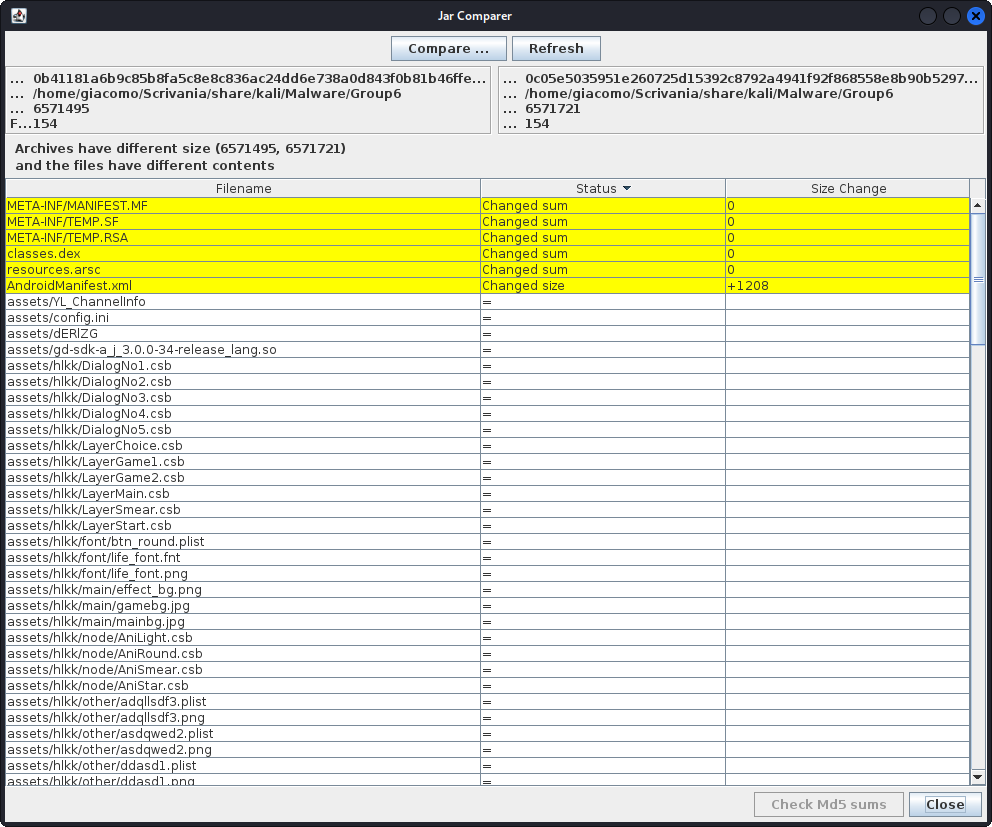
\includegraphics[width=1\textwidth]{./images/screenshot/jarcompare/jarCompare.png}
    \caption{jarCompare output}
    \label{fig:jarCompare}
\end{figure}

From this point forward we will always reference the \texttt{0c05..} sample file and its content when speaking about this virus family and, if there will be any differences with the other samples, they will be pointed out.

\section{Static Analysis}

As with SanaSystem, we firstly fed the obtained APK to virus total and got the following result shown in Fig. \ref{fig:MaidReview}.
\begin{figure}[h!]
\centering
    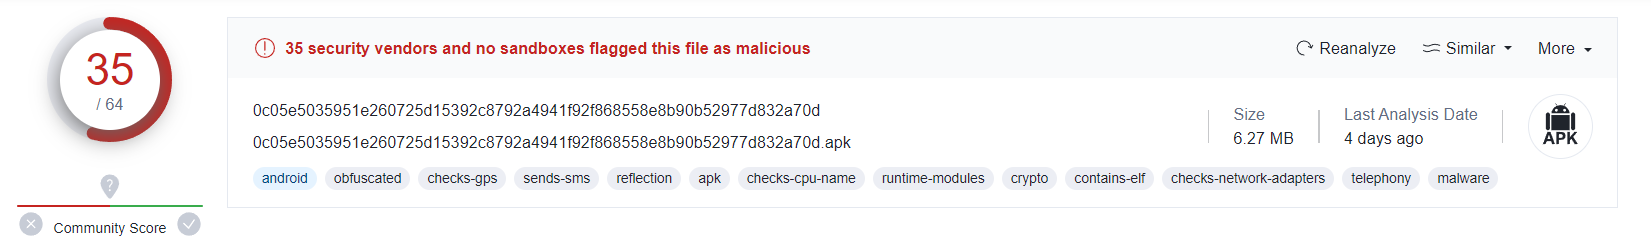
\includegraphics[width=1\textwidth]{./images/screenshot/NaughtyMaid/Review.png}
    \caption{Virus total review}
    \label{fig:MaidReview}
\end{figure}

In addition, the \texttt{0c40..} file received a score of 33/59, this indicates that, even if the files are practically the same, even small changes can affect the malware fingerprint which changes its detectability from anti-viruses. In particular a common anti-malware such as MalwareBytes was not able to recognize the software as malicious in every case. As show in Fig. \ref{fig:MaidDetection} the virus is categorized as trojan.smsreg/andr same as the other ones except for 0c40 which is classified as trojan.smsreg/smspay. The first one identifies an app disguised as a legit one with the malicious goal of collecting user and phone data, the second one identifies an app whose goal is to subscribe the phone to premium sms services and hide its functionality by deleting the incoming malicious sms. As previously stated the 4 files are basically the same malware and this difference in categorization implies a high range in malicious activity, this is also confirmed by the permission required shown in Fig. \ref{fig:MaidPermission}. In addition some permission are not shown by virus total so we decided to list the most suspicious not present in the virus total one:
\begin{itemize}
	\item read\textunderscore external\textunderscore storage
	\item read\textunderscore logs
	\item get\textunderscore account
	\item write\textunderscore settings
\end{itemize}

\begin{figure}[h!]
\centering
    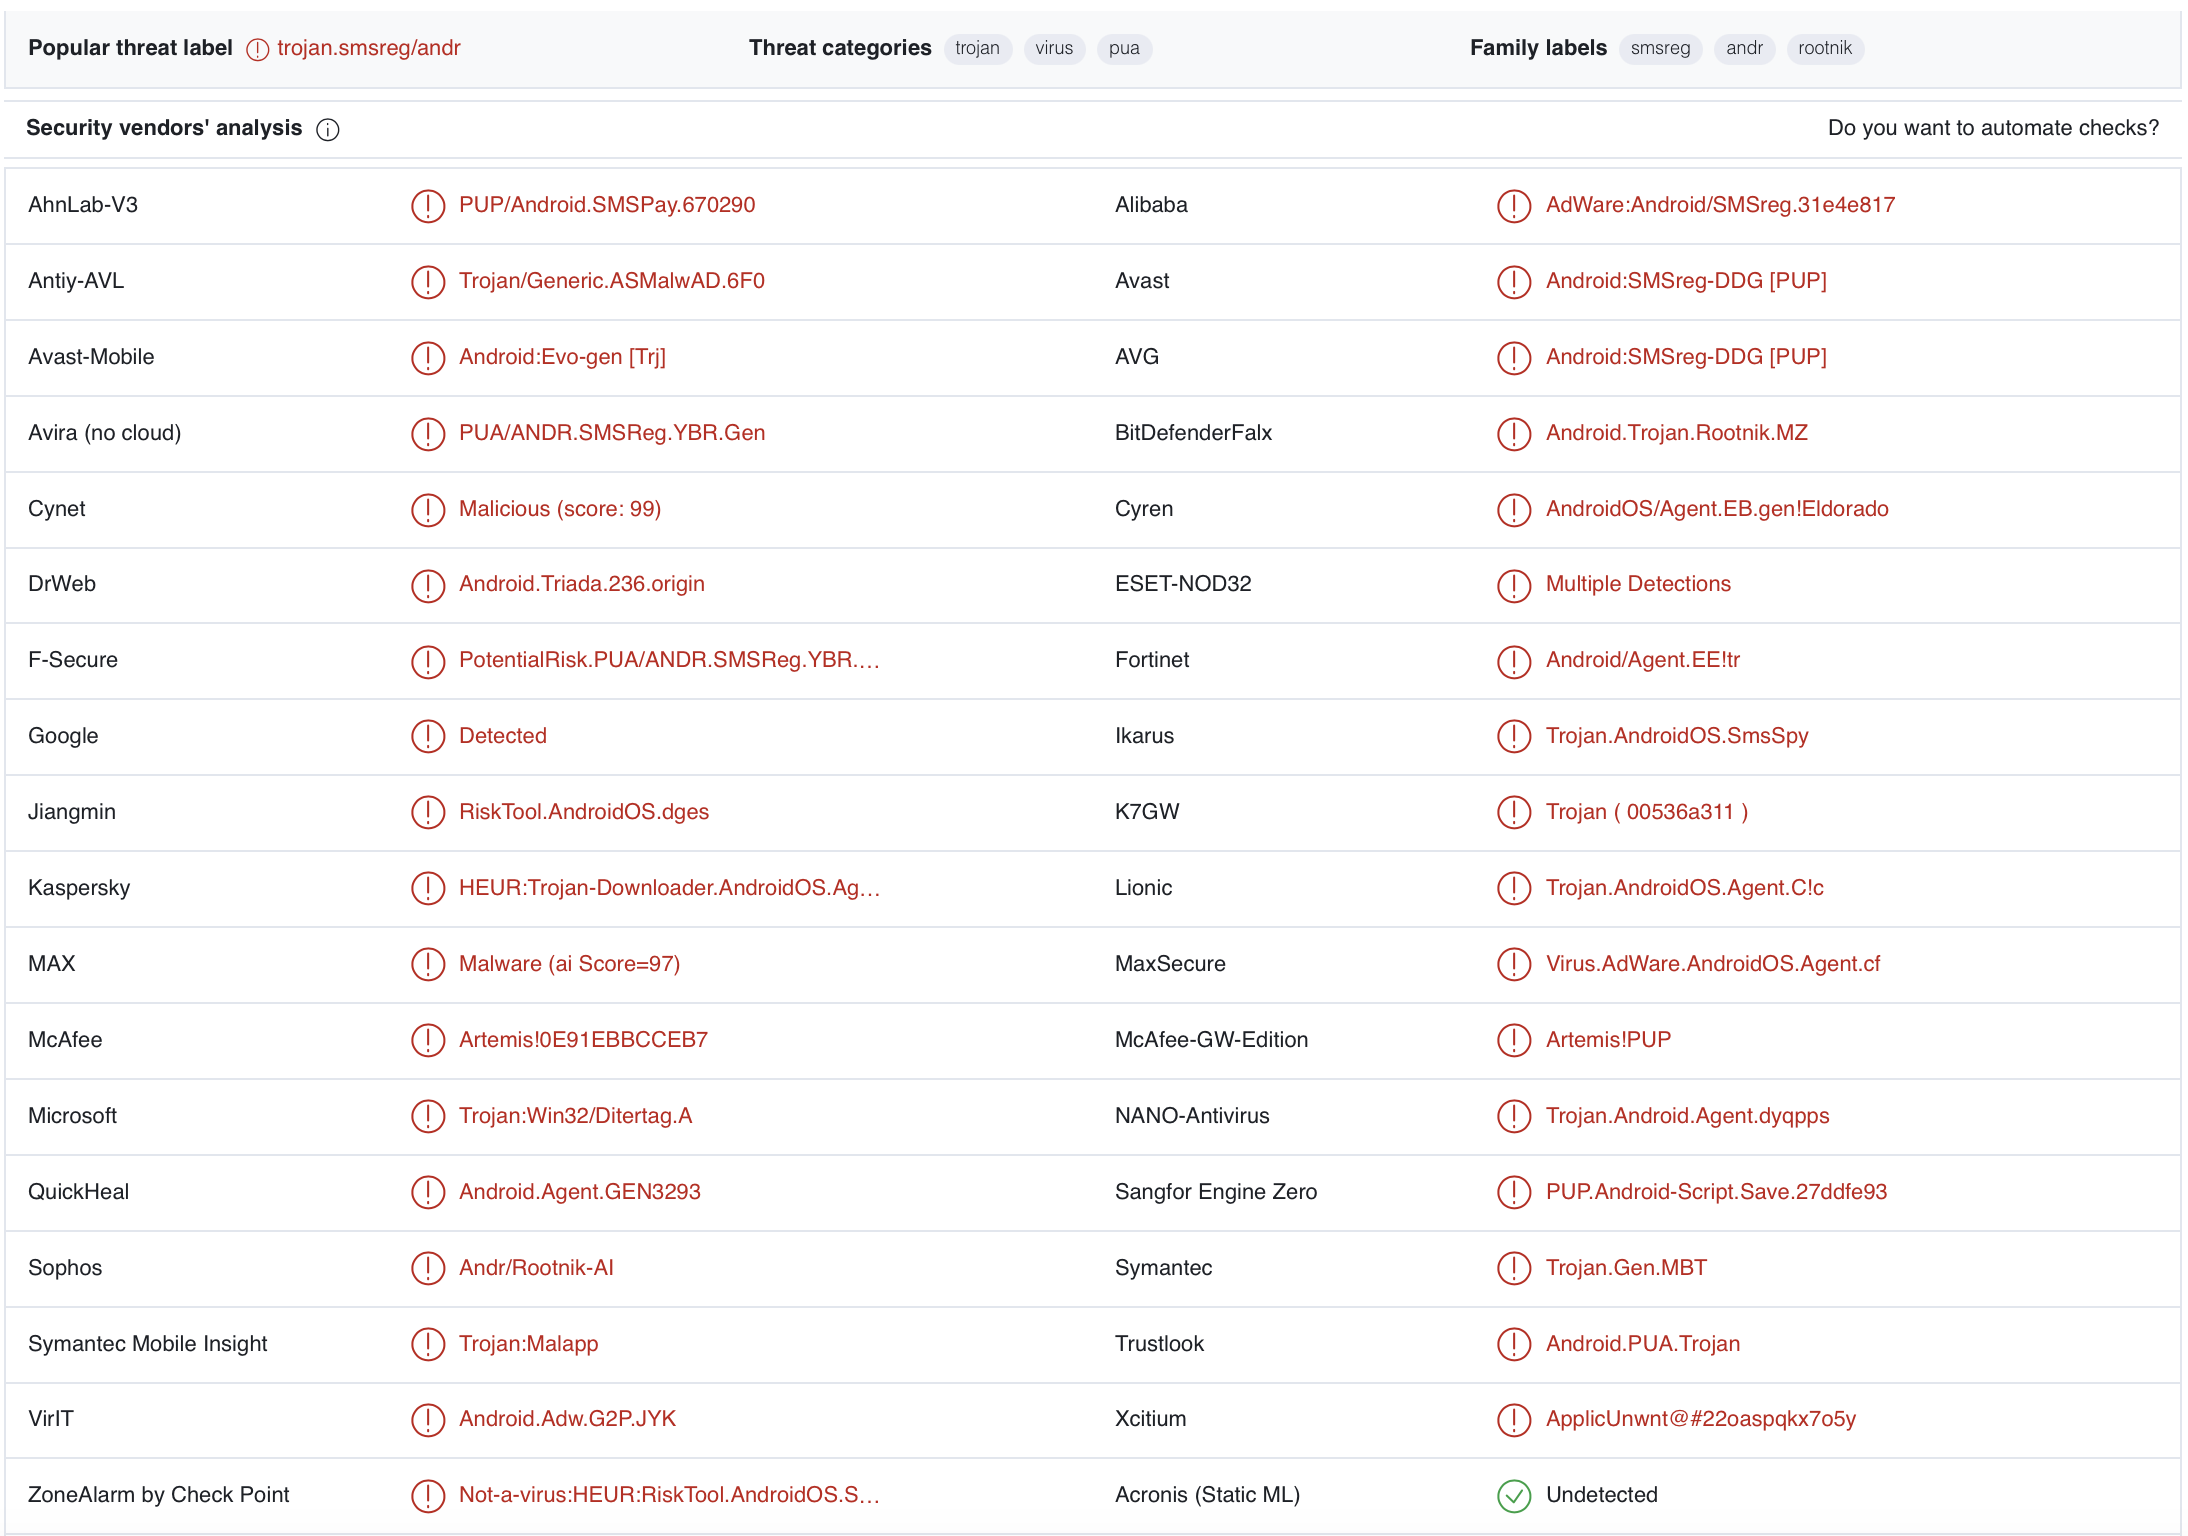
\includegraphics[width=1\textwidth]{./images/screenshot/NaughtyMaid/Detection.png}
    \caption{Virus total detection}
    \label{fig:MaidDetection}
\end{figure}

\begin{figure}[h!]
\centering
    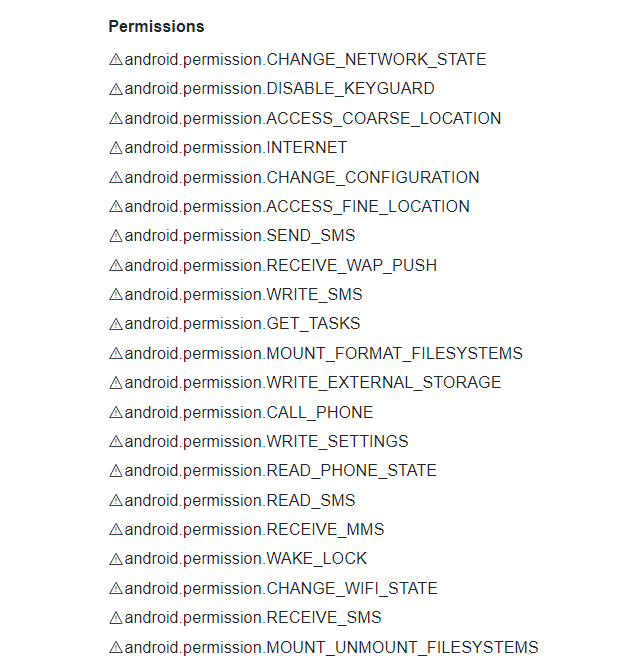
\includegraphics[width=0.5\textwidth]{./images/screenshot/NaughtyMaid/Permission.png}
    \caption{NaughtyMaid permission}
    \label{fig:MaidPermission}
\end{figure}

\subsection{URL and domains}
MobSF also indicated the presence of many hardcoded URL and relative domains Fig. \ref{fig:MaidDom1} \ref{fig:MaidDom2} \ref{fig:MaidDom3} \ref{fig:MaidDom4} \ref{fig:MaidDom5}. Many of them are located in China and, after a quick check with a DNS lookup and an IP lookup tools, it was revealed that other domains not identified by MobSF are located there. Others were misidentified and placed in European countries such as \emph{alog.umeng.com} that was signaled to be hosted in Frankfurt when in reality it resides in Honk Kong at the time of writing this report. 

Regarding the URLs there are too many to be presented in a single list so we decided to report the most suspicious ones, please note that these may be more malicious URLs, however these four are those with the most suspicious names.
\begin{itemize}
	\item http://118.85.194.4:8083/iapSms/ws/v3.0.1/mix/billing
	\item http://139.129.132.111:8001/CrackCaptcha/GetCaptchaValue.aspx
	\item http://pay.918ja.com
	\item http://vpay.api.eerichina.com/api/payment
\end{itemize}

\begin{figure}[h!]
\centering
    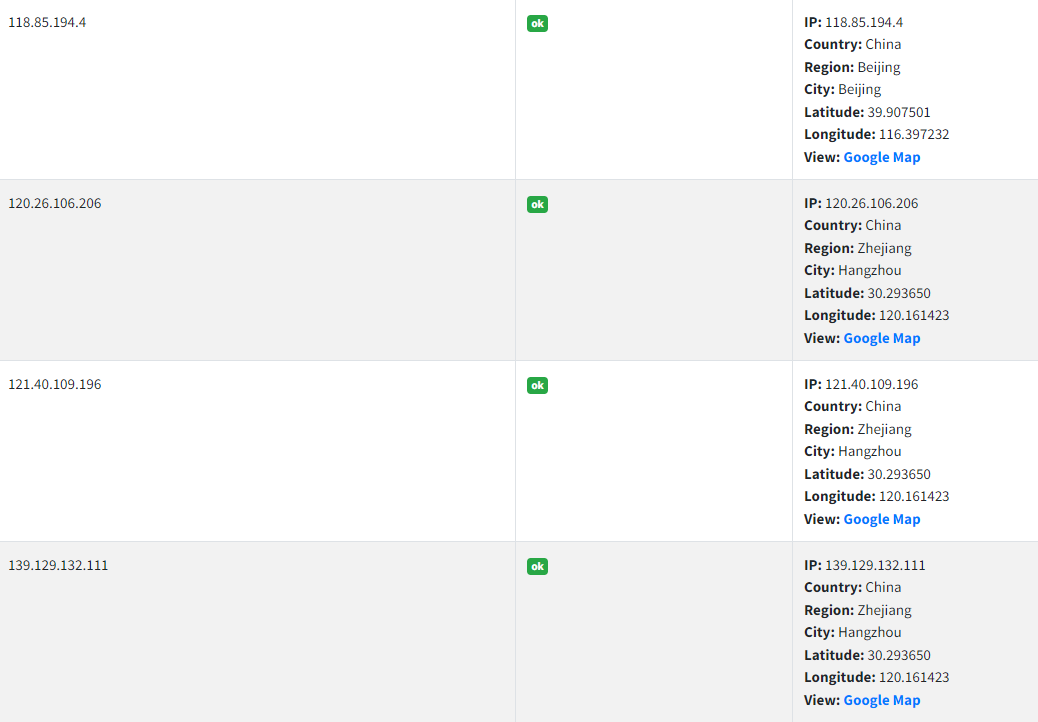
\includegraphics[width=1\textwidth]{./images/screenshot/NaughtyMaid/Domain1.png}
    \caption{Domain from MobSF 1}
    \label{fig:MaidDom1}
\end{figure}

\begin{figure}[h!]
\centering
    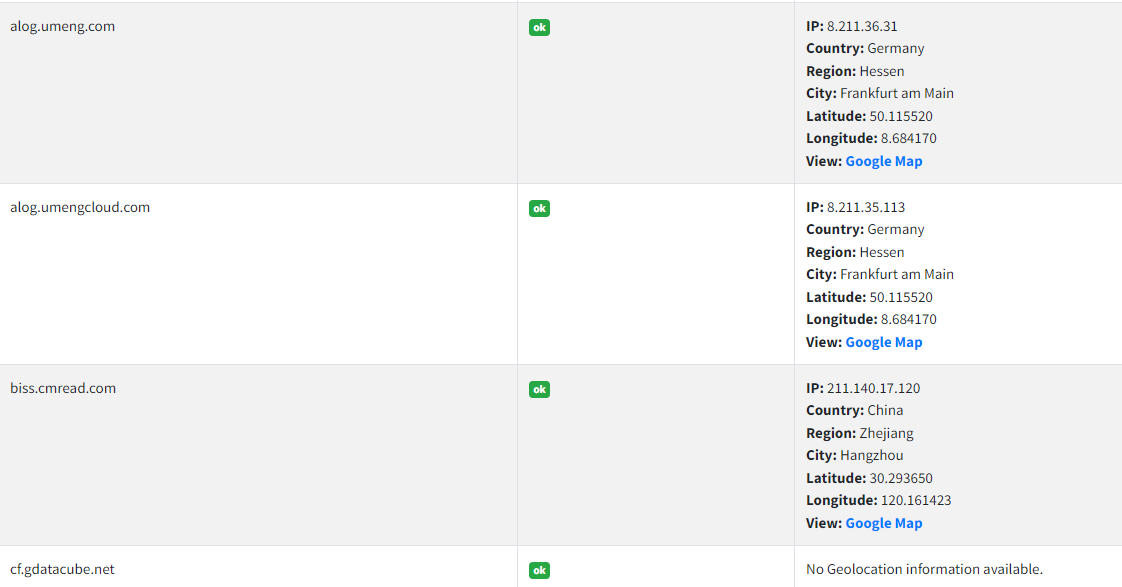
\includegraphics[width=1\textwidth]{./images/screenshot/NaughtyMaid/Domain2.png}
    \caption{Domain from MobSF 2}
    \label{fig:MaidDom2}
\end{figure}

\begin{figure}[h!]
\centering
    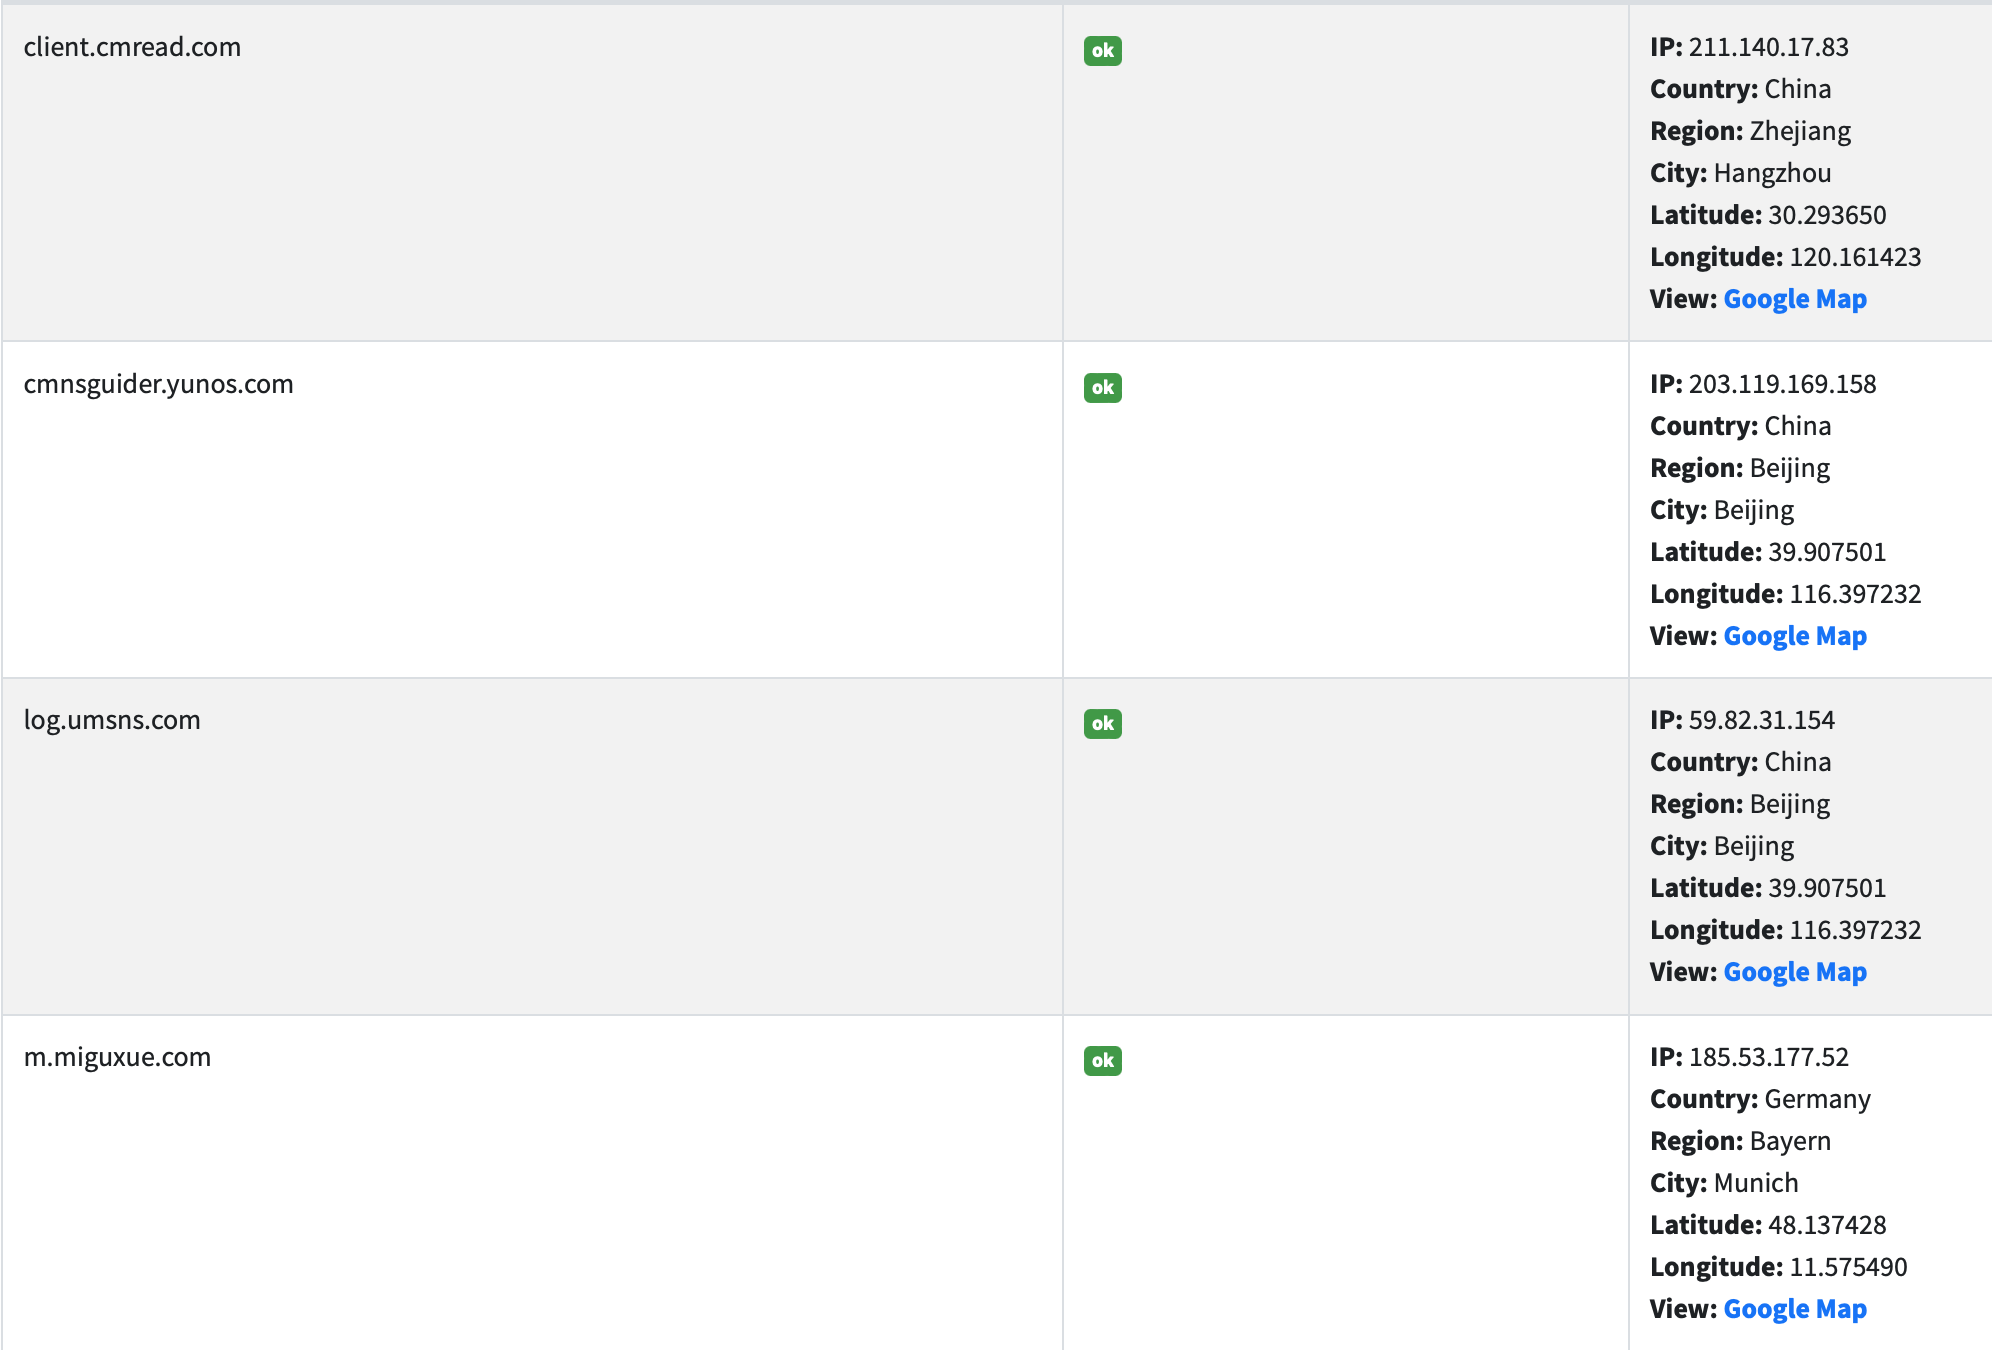
\includegraphics[width=1\textwidth]{./images/screenshot/NaughtyMaid/Domain3.png}
    \caption{Domain from MobSF 3}
    \label{fig:MaidDom3}
\end{figure}

\begin{figure}[h!]
\centering
    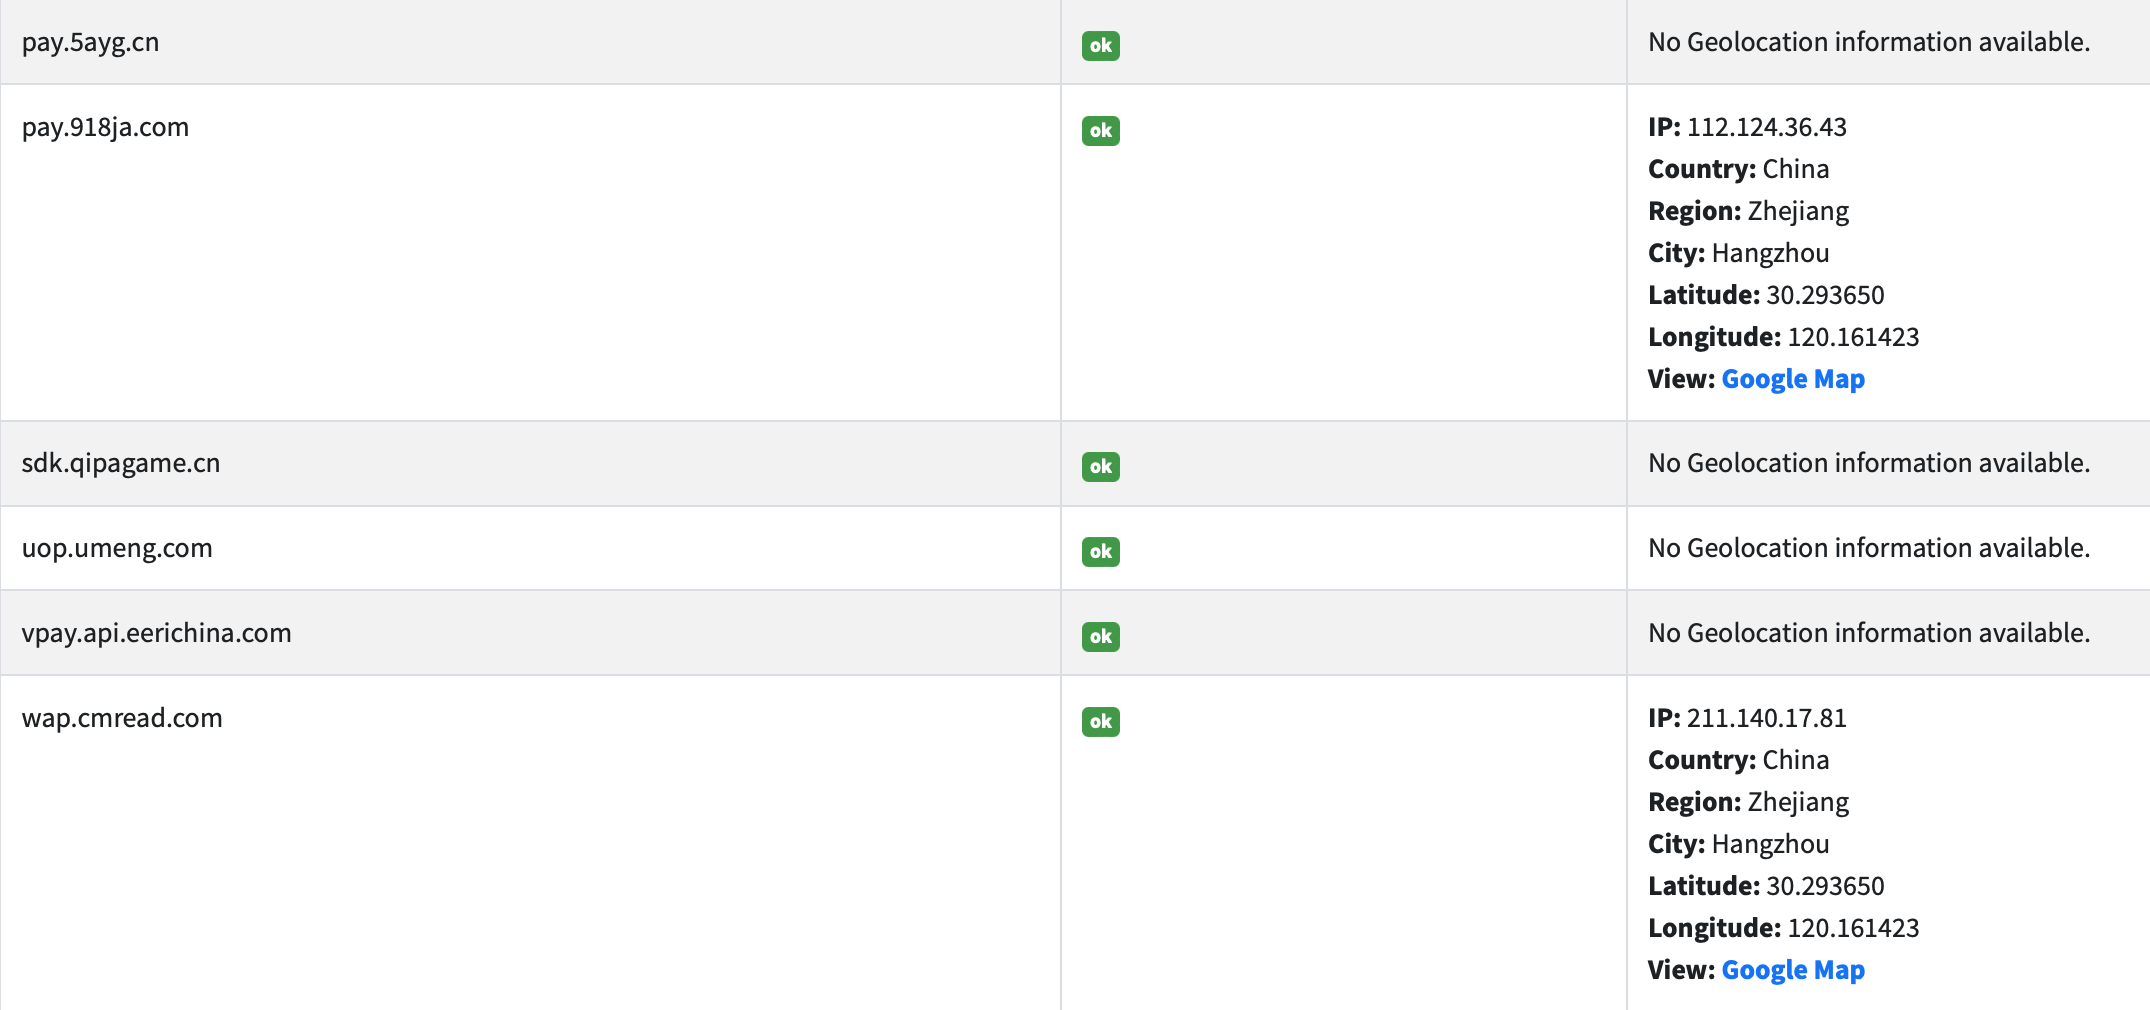
\includegraphics[width=1\textwidth]{./images/screenshot/NaughtyMaid/Domain4.png}
    \caption{Domain from MobSF 4}
    \label{fig:MaidDom4}
\end{figure}

\begin{figure}[h!]
\centering
    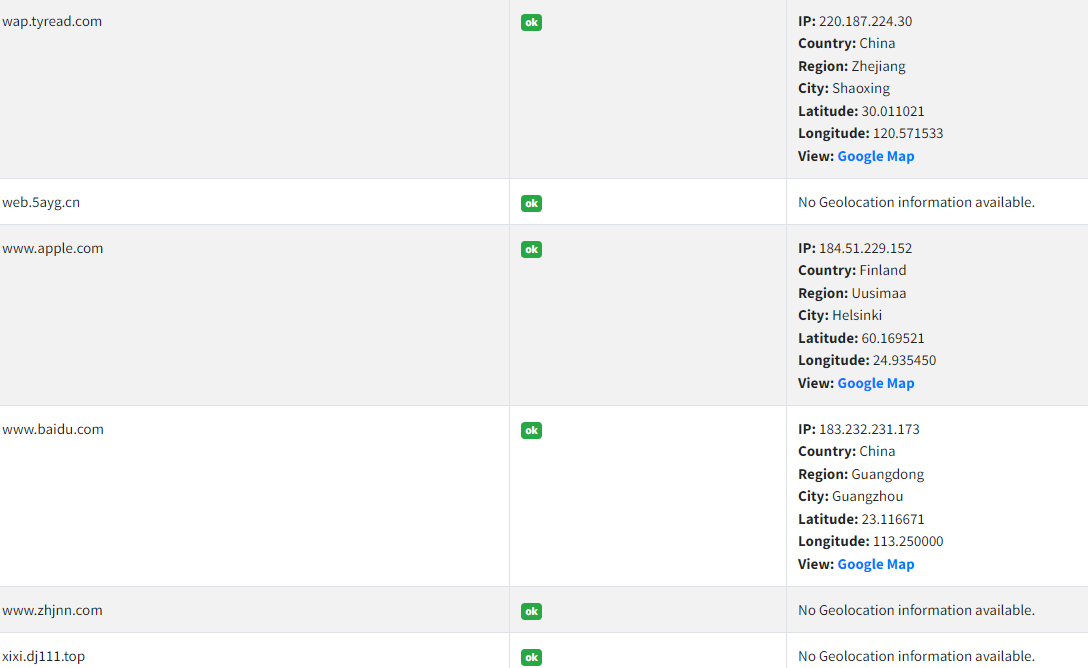
\includegraphics[width=1\textwidth]{./images/screenshot/NaughtyMaid/Domain5.png}
    \caption{Domain from MobSF 5}
    \label{fig:MaidDom5}
\end{figure}

In addition MobSF signal the presence of a tracker (Fig. \ref{fig:MaidTracker}) whose info can be consulted on exodus \footnote{\url{https://reports.exodus-privacy.eu.org/it/trackers/119/}}, in particular this tracker is associated with the \texttt{alog.umeng.com} domain present in Fig. \ref{fig:MaidDom2}

\begin{figure}[h!]
\centering
    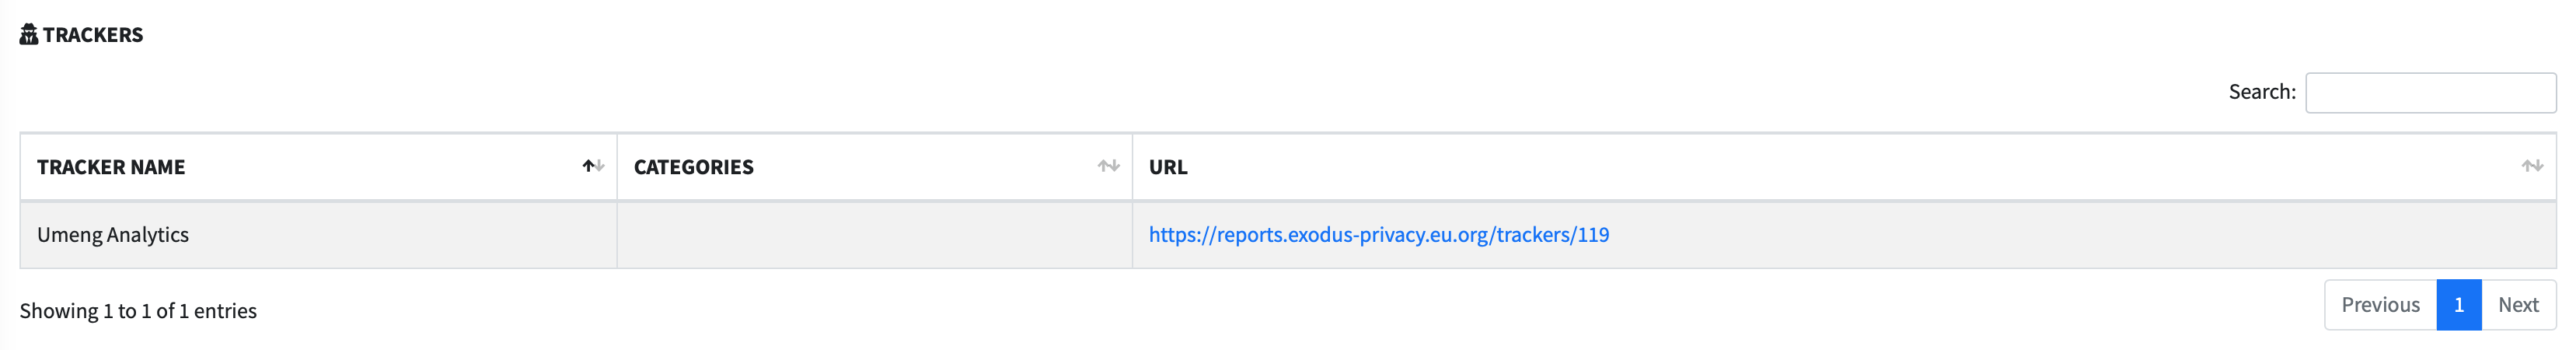
\includegraphics[width=1\textwidth]{./images/screenshot/NaughtyMaid/Tracker.png}
    \caption{Tracker signaled by MobSF}
    \label{fig:MaidTracker}
\end{figure}

\subsection{Code analysis}
As can be seen in Fig. \ref{fig:CodeOrganization} the code is very obfuscated, since the classes do not contains significant names, most of them are a single character and there are lot of folders. 
\begin{figure}[h!]
\centering
    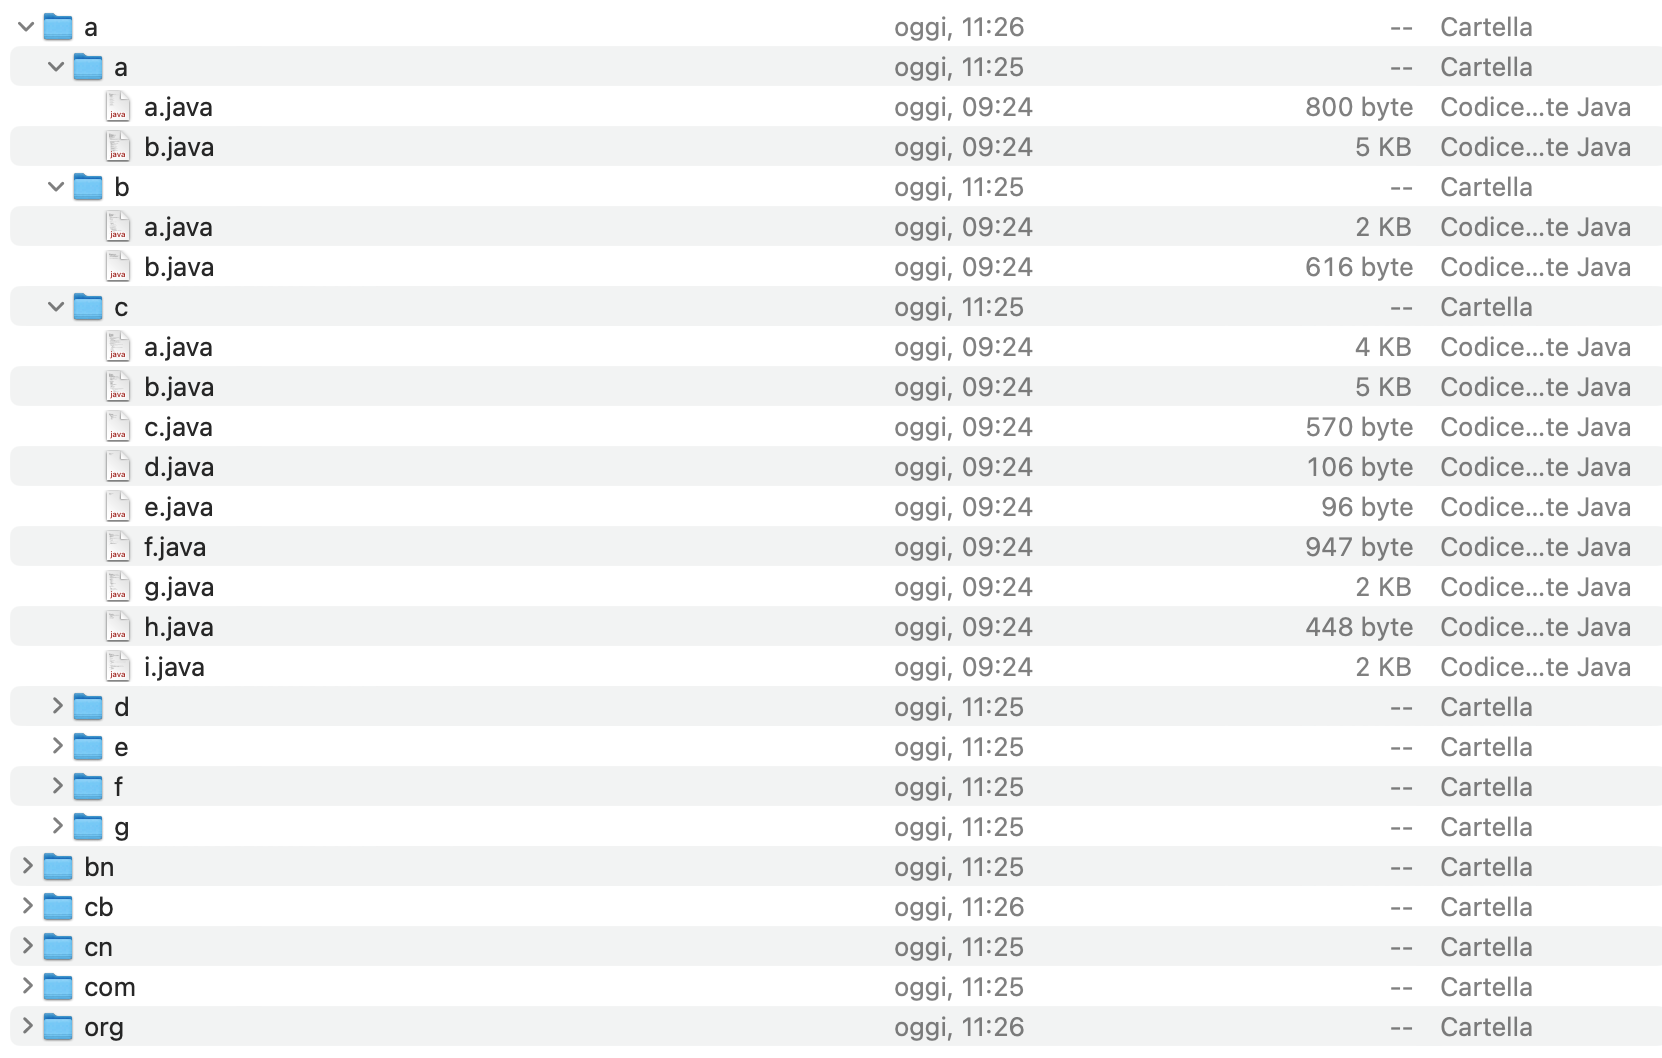
\includegraphics[width=1\textwidth]{./images/screenshot/NaughtyMaid/PackageStructure.png}
    \caption{Structure of the package}
    \label{fig:CodeOrganization}
\end{figure}

\subsubsection{AppActivity}
Thanks to VirusTotal we were able to rapidly identify the main activity, called \texttt{AppActivity}, that is placed in the \texttt{org.cocos2dx.cpp} package. Cocos2d-x \footnote{\url{https://github.com/cocos2d/cocos2d-x}} is a multi-platform framework for building 2d games, interactive books, demos and other graphical applications. 
The class extends \texttt{Cocos2dxActivity} which extends Activity class of Android. When the activity is launched, the \texttt{onCreate} method is called. First there is a check if the activity is the root of the task, if not there is another check on the category of the intent, and if the \texttt{mainIntent} has a launcher category and the action of intent is main, the activity is stopped. The reason behind this behaviour might be related to an anti-debugging technique: the process asserts it being run from the launcher and if it senses it is a child process, maybe of a debugger, it stops its execution.

\begin{figure}[h!]
\centering
    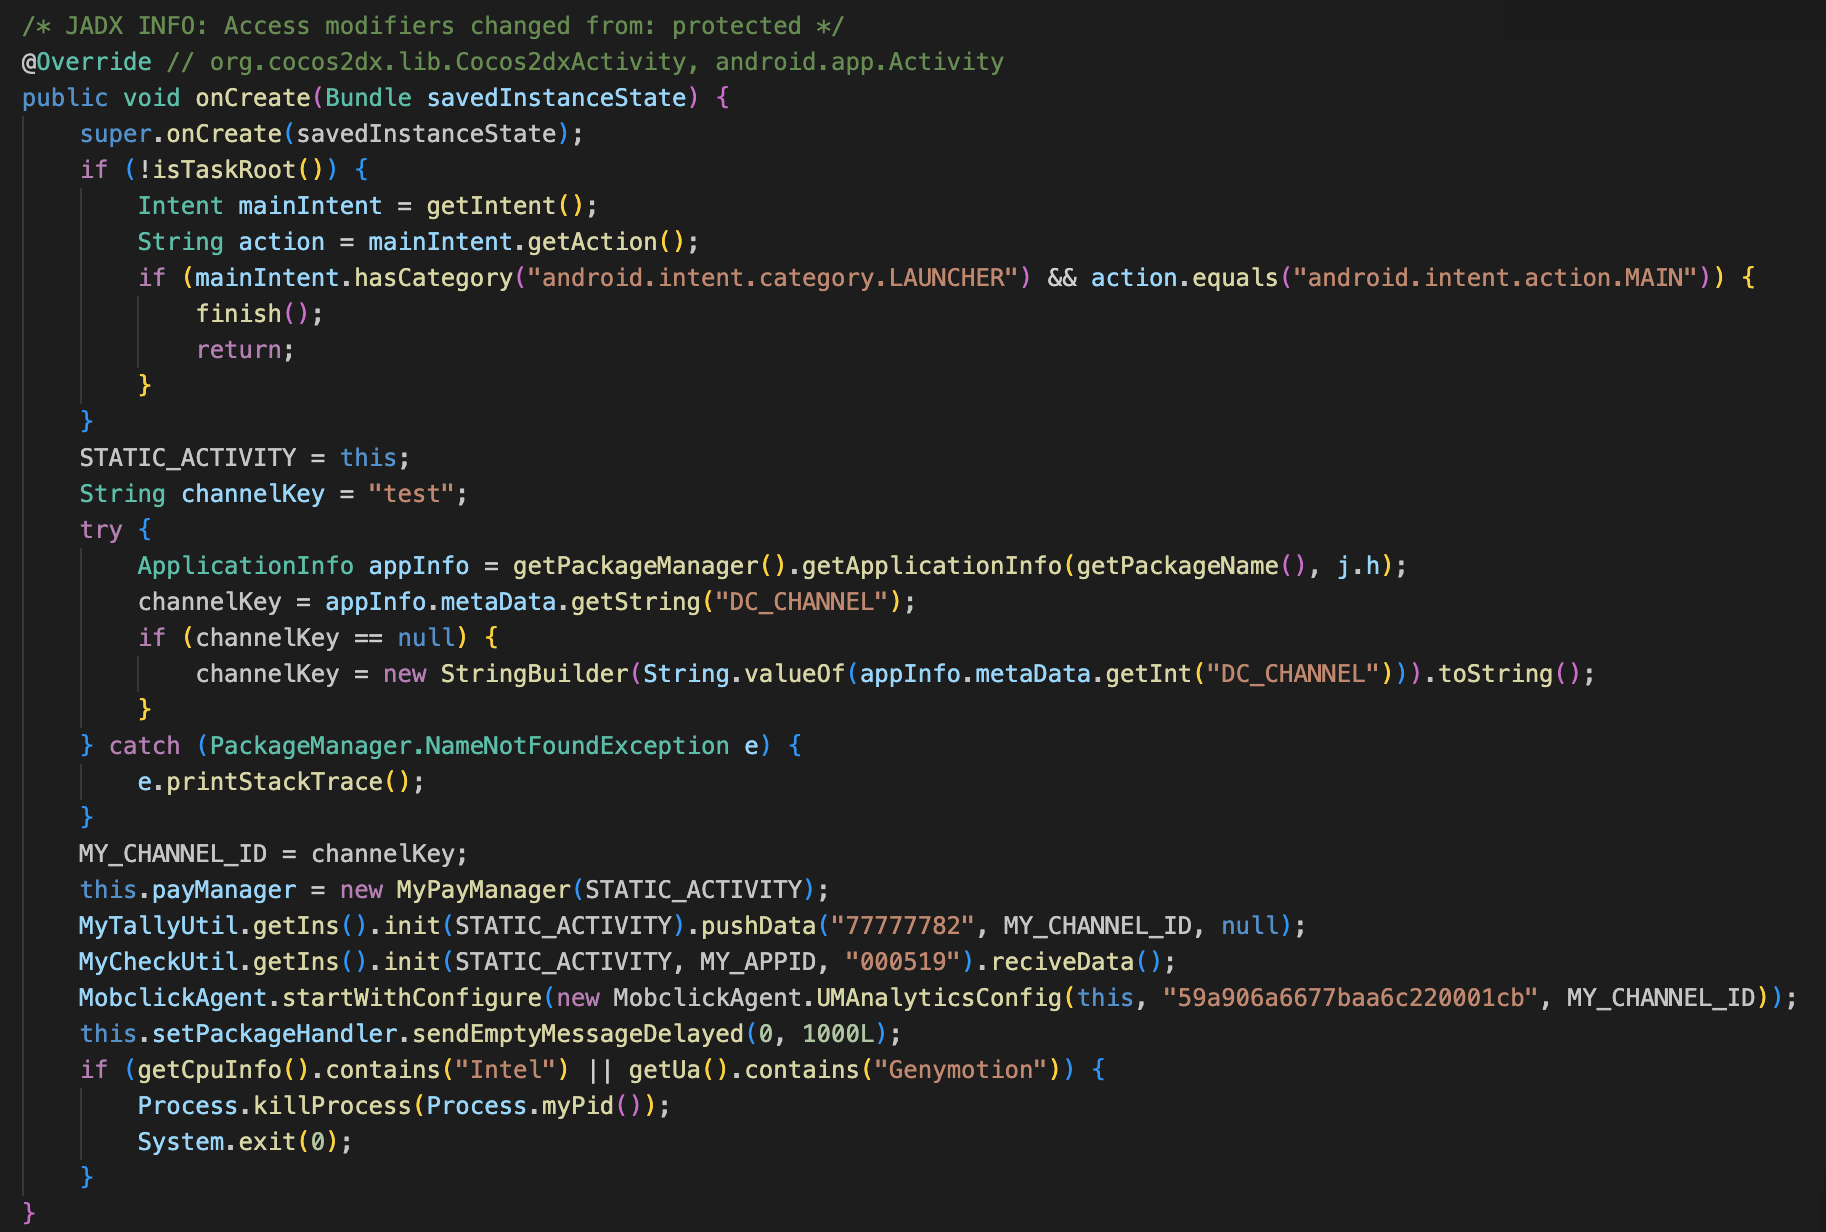
\includegraphics[width=1\textwidth]{./images/screenshot/NaughtyMaid/AppActivity.png}
    \caption{AppActivity:onCreate}
    \label{fig:AppActivityOnCreate}
\end{figure}

Then an object MyPayManager is created and the init method of MyTallyUtil and MyCheckUtil are called. At the end of the method there is also an interesting behavior, there is a check against the name of the CPU, with \texttt{getCPUInfo()} (Fig \ref{fig:AppActivitygetCPUInfo}) and the manifacturer, with \texttt{getUa()} (Fig \ref{fig:AppActivitygetUa}). \texttt{getCPUInfo()} basically executes the command "cat /proc/cpuinfo", while \texttt{getUa()} gets information of the model, the manifacturer and the brand. If the cpu string contains "Intel" or the manifacturer string contains "Genymotion" the activity kills the current process. This is like a protection measure that the author inserts, so that the app can't run on a virtual environment. 
\begin{figure}[h!]
\centering
    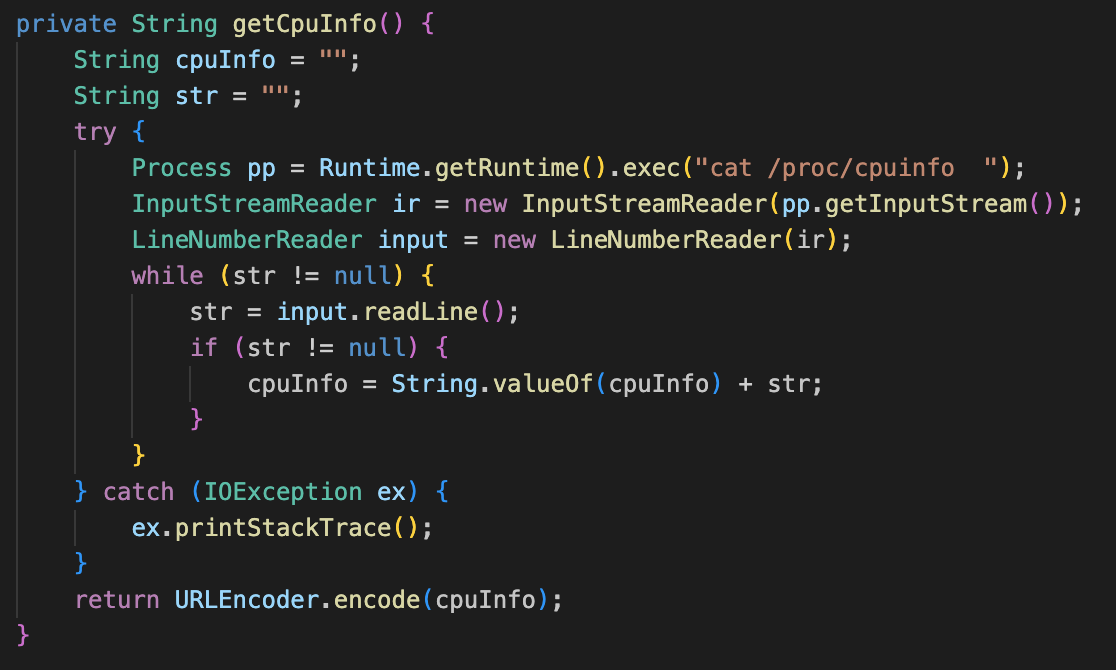
\includegraphics[width=1\textwidth]{./images/screenshot/NaughtyMaid/getCPUinfo.png}
    \caption{AppActivity:getCPUInfo}
    \label{fig:AppActivitygetCPUInfo}
\end{figure}
\begin{figure}[h!]
\centering
    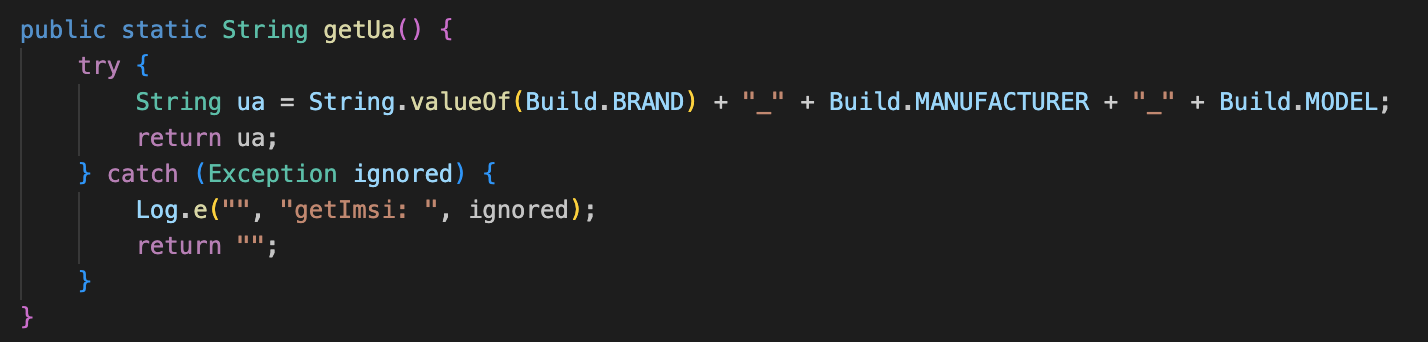
\includegraphics[width=1\textwidth]{./images/screenshot/NaughtyMaid/getUa.png}
    \caption{AppActivity:getUa}
    \label{fig:AppActivitygetUa}
\end{figure}

\subsubsection{myPayManager}
\begin{figure}[h!]
\centering
    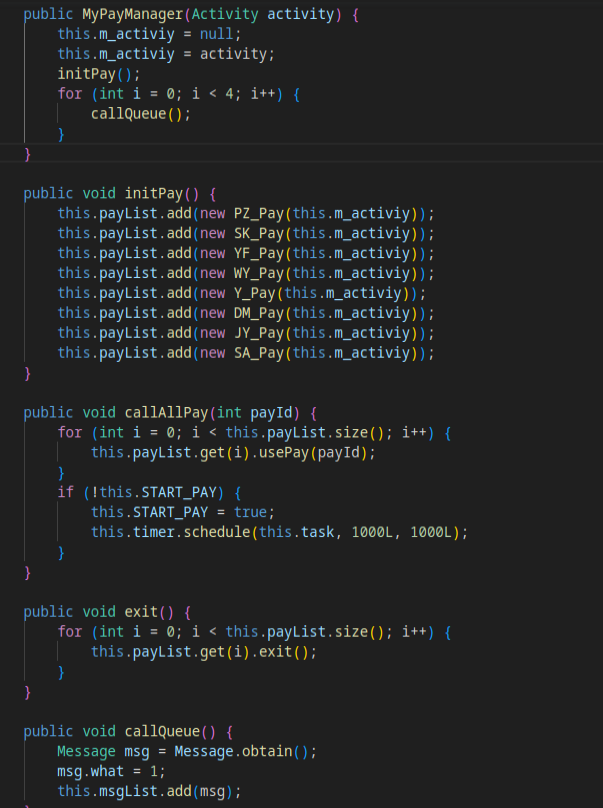
\includegraphics[width=1\textwidth]{./images/screenshot/NaughtyMaid/myPayManager.png}
    \caption{myPayManager}
    \label{myPayManager}
\end{figure}

